% Survey.tex
%==============================================================================
\section{Research Directions}
\label{sec:survey}

\noindent 
This section presents the research issues which will be addressed in our thesis. We elaborate a comparison framework under the perspective of the performance of the execution engines of the integration platforms. Then we apply our framework to ten known platforms and from the results we extract research problems.
%==============================================================================
\subsection{{Framework}}
\label{subsec:framework}
%==============================================================================

\noindent 
Our framework is composed of two dimensions: efficiency and fairness execution, which contain properties that can have an impact on the performance of the runtime system. The dimensions and their respective properties are detailed below.

%==============================================================================
\subsubsection{{Efficiency}}
\label{subsubsec:efficiency}
%==============================================================================
This dimension relates to improving the efficiency of the runtime system to process a message, which can also be seen as increasing the average number of messages processed by time unit. It comprises the following properties that relates to the capacity of reducing the real-time demanded by the integration solution to completely process a message:
\begin{itemize} 
\item \textbf{Designed for Multi-core}. Multi-core programming has to be carried out in order to take full advantage of multiple cores available in the hardware processors. This property indicates whether the runtime system has been developed to take advantage of multi-core or not. Multiple cores work together to increase the capability of process multiple tasks or increase the performance of the system by operating on multiple instructions simultaneously in an efficient manner. It can take the following values: \texttt{yes} or \texttt{no}. \texttt{yes} indicates the runtime system was developed to take advantage of multi-core hardware, otherwise, the value is \texttt{no}.

\item \textbf{Thread Pool Configuration}. The runtime system allows to configure one or more pools of threads to the integration solution, and this property indicates how threads are managed in these pools. This property may take the following values: \texttt{fixed}, \texttt{limited} or \texttt{elastic}. \texttt{fixed} indicates that a thread pool is composed of a fixed number of threads, which is known at design time; \texttt{limited} indicates the number of threads in a thread pool can increase automatically during runtime until a threshold defined at design time is reached; \texttt{elastic}, indicates that the number of threads in a thread pool can automatically increase and decrease during runtime within a range of values defined at design time.
%
\item \textbf{Type of Message Storage in Process}. Messages can contain a huge amount of data, which will have an impact on the amount of memory required by channels inside the integration solution and depending on the type of storage it has an impact on the real-time execution. This property indicates whether the message is stored in memory, disk, or both. It may take the following values: \texttt{memory}, or \texttt{disk}, or both.
%
\item \textbf{Distributed Process Execution}. Indicates whether an integration solution can be divided and distributed to different machines to execute a set of correlated messages, promoting scalability. This property allows increasing the number of tasks executed per time unit in cases in which there is no dependency between the tasks, i.e., the input data of one task is the output data produced by another task. This property may take the following values: \texttt{yes} or \texttt{no}. \texttt{yes} indicates the runtime system takes advantage of scalability, otherwise, the value is \texttt{no}.
%	
\item \textbf{Thread Pool Creation}. Historical and current execution data can be used by runtime systems to make decisions during runtime, determining optimised strategies to create threads. This property indicates the way and stage at which thread pools can be created. This property may take the following values: \texttt{dynamic} or \texttt{static}. \texttt{dynamic} indicates that thread pool creation is done at runtime from data taken from the runtime system and indicates the need for a pool and \texttt{static} value indicates that the pool creation is done at design time by the software engineer.	
\end{itemize}
%
%==============================================================================
\subsubsection{{Fairness execution}}
\label{subsubsec:fairness}
%==============================================================================
\noindent
This dimension concerns to assignment of threads to tasks aiming at a fair execution of them to help to minimise the average time that a message takes to be processed in the integration solution. The following properties provide means that contribute to have a fair execution of tasks:
\begin{itemize}
% 	\item \textbf{Priority to task execution}. Indicates whether the runtime system allows tasks to have priority associated with them so that it affects the execution policy by the runtime system. This property may take the following values: \texttt{yes} or \texttt{no}. \texttt{yes} indicates the runtime system can deal with priority in tasks.
%	
\item \textbf{Starvation Detection}. Indicates whether the runtime system is endowed with the capacity to detect tasks that do not execute within an accepted time-frame. This property may take the following values: \texttt{yes} or \texttt{no}. \texttt{yes} indicates the runtime system can detect starvation, otherwise, \texttt{no}. 
%	
\item \textbf{Thread Pool Policy}. Indicates the strategy followed by the runtime system to assign the existing threads to the different tasks. This property may take the following values: \texttt{FIFO}, \texttt{priority} or \texttt{mapping}. \texttt{FIFO} means that the runtime system follows First-In-First-Out(FIFO) heuristic, in which the threads are being allocated the tasks in order that arrive, so that the first ones that arrive are attended to before; \texttt{priority} means that the runtime system allows tasks to have priority associated; and, \texttt{mapping} means that the scheduling policy follows a mapping based on a mathematical model or optimization method that allows finding an optimal scheduling policy by previously evaluating the integration solution.
%	
\item \textbf{Task Complexity}. Indicates whether the runtime system takes into consideration the computational complexity of tasks to allocate threads. This property may take the following values: \texttt{yes} or \texttt{no}. \texttt{yes} indicates that the runtime system knows the computational complexity of each of the tasks and this can be utilised in the decision in choosing the order of execution of tasks, such as tasks of less computational complexity can be executed first, as soon as possible; otherwise, \texttt{no}.
%
\item \textbf{Execution Model}. Indicates the execution model implemented by the runtime system, which deals with the granularity of the execution of tasks. This property may take the following values: \texttt{process-based}, \texttt{task-based} or \texttt{hybrid}. In the \texttt{process-based} model, the runtime system controls process instances as a whole, i.e., there are no means that it can interact with the internal tasks; contrarily, in the \texttt{task-based} model, the runtime system may control both process instances and their internal tasks. In the \texttt{hybrid} model, the runtime system will adopt the model that better fits the execution profile about some predefined parameters, such as message input rate, the number of processors, average message size. 
%
\item \textbf{Throttling Controller}. Indicates whether the runtime system allows controlling the rate of incoming messages on input ports. If the input rate exceeds the processing capacity of the initial tasks, the runtime system can adopt suitable policies, such as, refusing new messages on passive ports or tuning the frequency of the pooling in the active ports. This property may take the following values: \texttt{yes} or \texttt{no}. \texttt{yes} indicates that the runtime system can control the rate of incoming messages, that is, it has a throttling controller; otherwise, \texttt{no}. 
\end{itemize}

%==============================================================================
\subsection{{Comparison}}
\label{subsec:comparasion}
%==============================================================================
\noindent
We selection some popular integration platforms to apply the comparison framework. For this, we rely in the methodology the integrative literature review, which includes the following steps: identification of the theme and elaboration of the inclusion and exclusion criteria of articles, construction of an instrument for collection of relevant data of the articles found, evaluation and analysis of the articles selected in the research, interpretation and discussion of the results obtained and presentation of the review.

We search the databases: IEEE Xplore, ACM Digital Library, Scorpus, using the keywords: "runtime system" and "execution engine". The inclusion criteria were: articles published in English, abstracts available in the chosen databases, availability of the same in full, published between the period from 2012 to 2017, not to restrict the area of knowledge used by the runtime systems.
We revised the Gartner report~\cite{gartner2016,guttridge2017} and Ovum report~\cite{sharma2017} for integration platforms and also made an exhausting search on the Web to build a list of candidate integration platforms. 

We have adopted the following criteria to select the integration platforms: they must follow the pipes-and-filters architectural style~\cite{alexander1977} and support enterprise integration patterns (EIPs)~\cite{hohpe2004}.
%and have their code under an open source license. 
The pipes-and-filters architecture style suggests dividing a task into smaller tasks, which are connected through communication channels in the message flow of the application, and the output of one task is the input to the next. In this architectural style, the computational components that perform an atomic task on inbound messages to route, transform or modify them and produce one or more outbound messages which are sent to the next filter by means of a communication channel, called pipe. We apply the aforementioned criteria and then we exclude those that did not meet the criteria or had enough documentation to allow applying our framework.

Enterprise integration patterns are conceptual standards identified and documented by Hohpe and Woolf~\cite{hohpe2004}, such standards have become a benchmark amongst software engineers and have inspired several integration platforms~\cite{isen2010,dossot2014,fisher2012,frantz2012}. EIPs document a set of best-practices to implement tasks which help to solve recurrent application integration problems.

We have analysed the runtime system of Mule~\cite{dossot2014}, Camel~\cite{isen2010}, Spring Integration~\cite{fisher2012}, Synapse~\cite{rademakers2008,jayasinghe2011}, Fuse~\cite{russell2012}, ServiceMix~\cite{konsek2013}, Petals ESB~\cite{surhone2010}, Jitterbit~\cite{russell2012_1} and WSO2 ESB~\cite{indrasiri2016}. It is important to note that the component SE Camel embeds the Apache Camel routing runtime system to execute enterprise integration patterns (EIP) in Fuse, ServiceMix and Petals, therefore, some properties have the same values.

The comparison of the runtime systems, regarding proprieties related to efficiency and fairness execution are summarised in Table~\ref{tab:comparison}.
\begin{table*}[htbp]
	\centering
	\caption{Comparison between runtime systems.}
    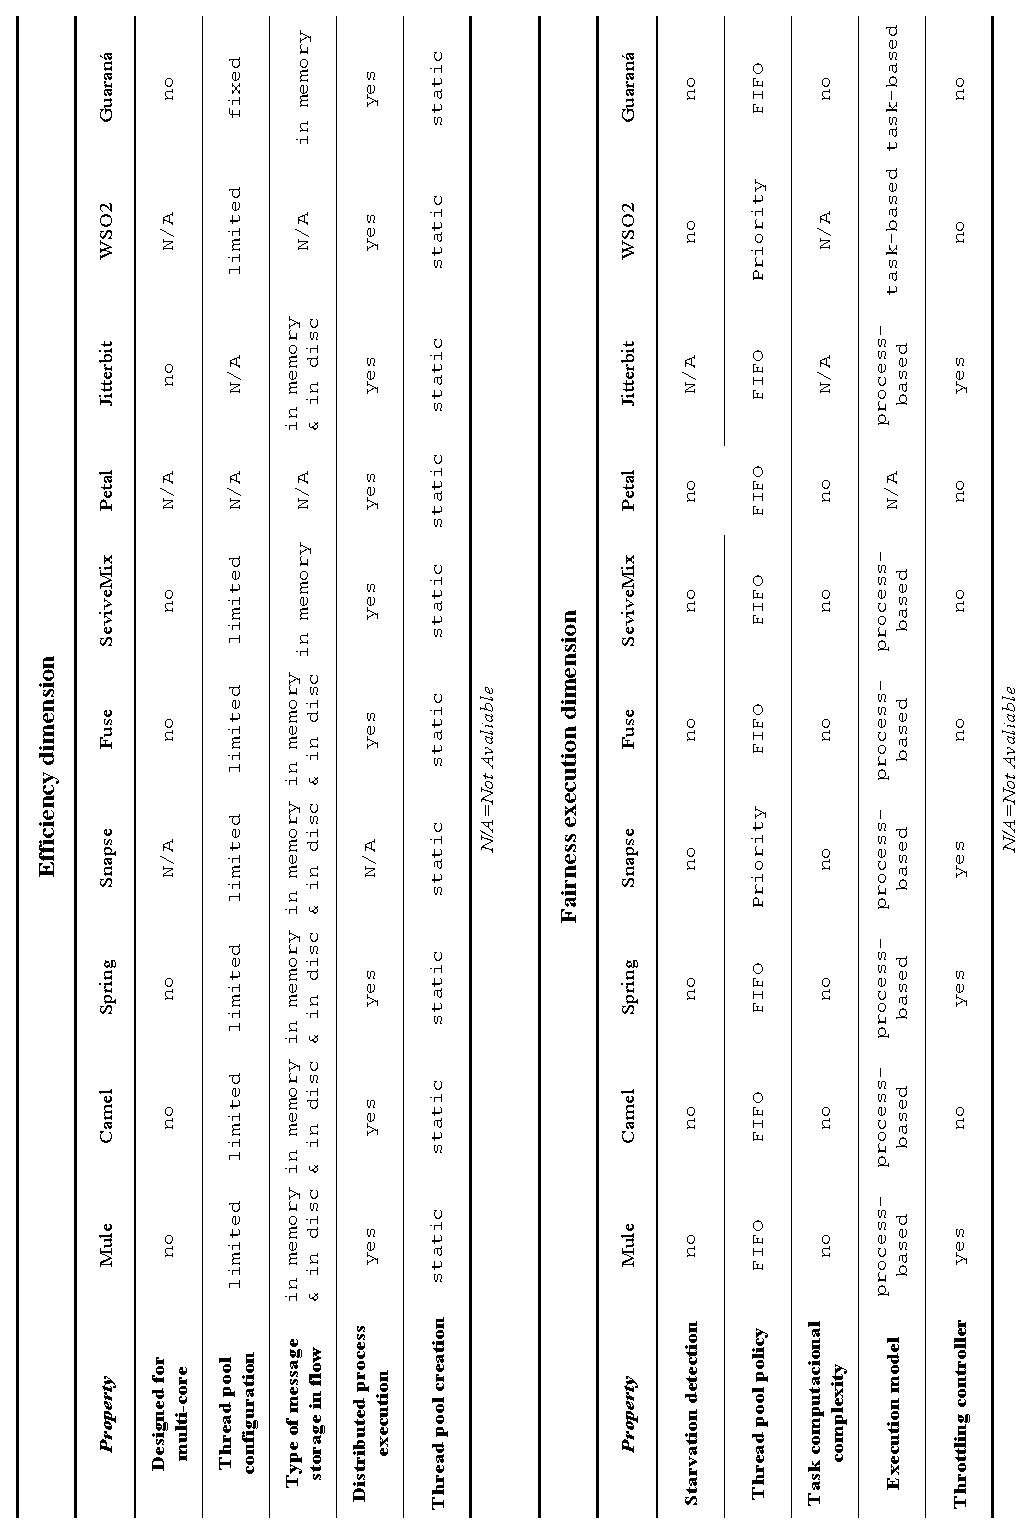
\includegraphics[scale=0.8]{./figs/table_dimensions_v.eps}
	%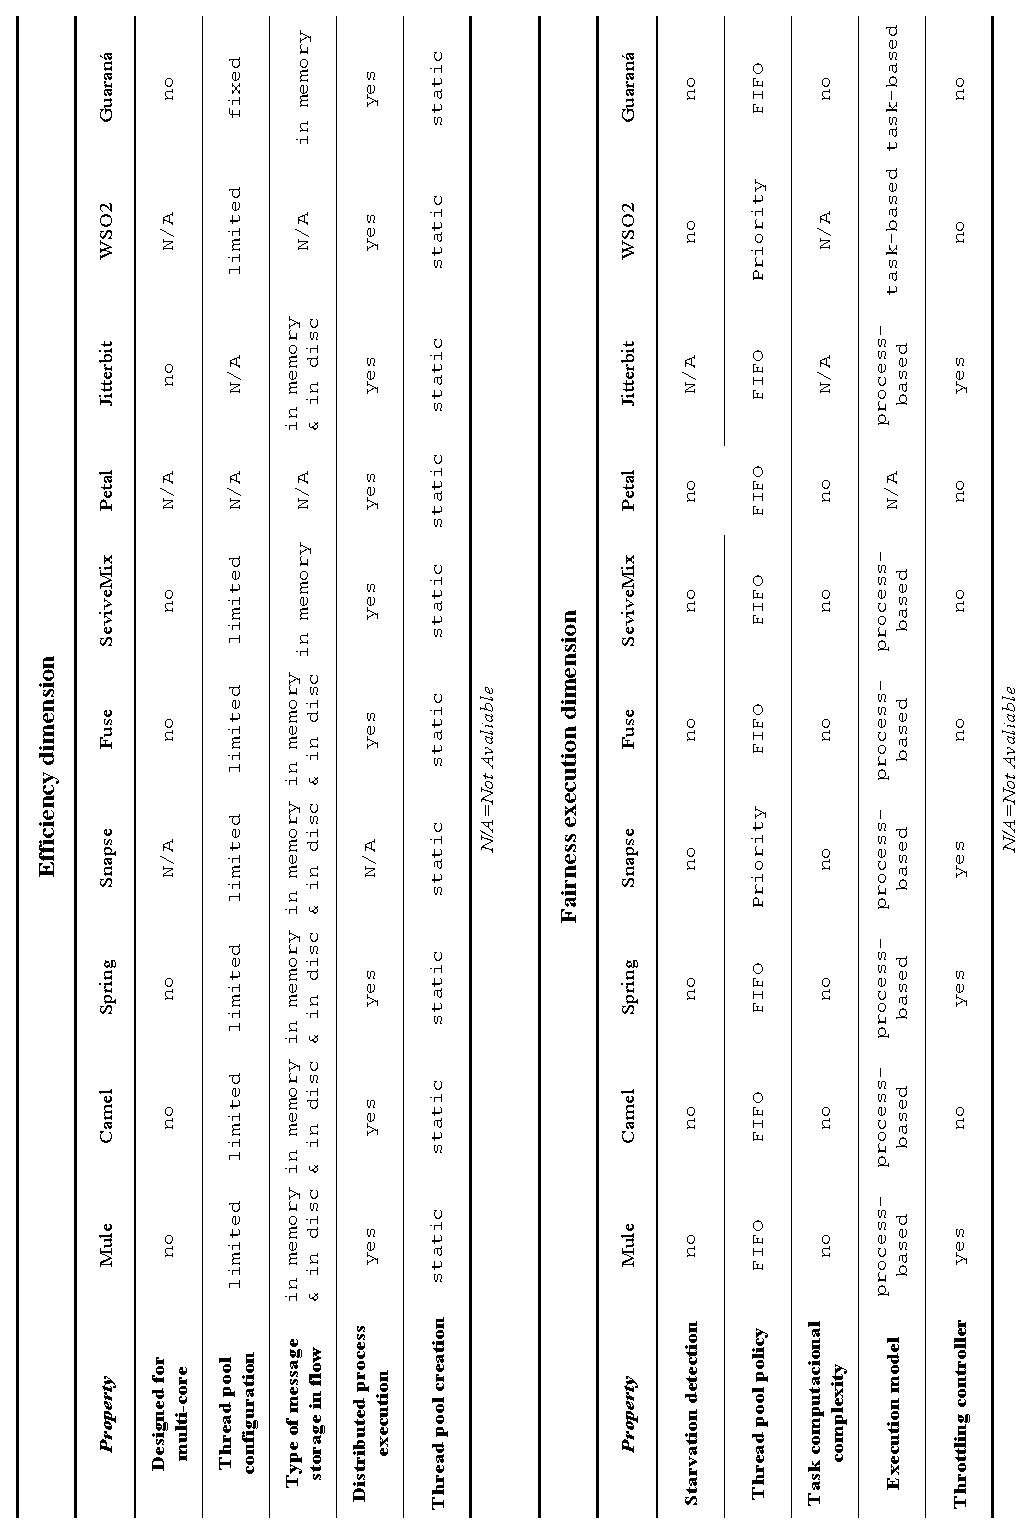
\includegraphics[width=\linewidth]{./figs/table_dimensions_v.eps}
	\label{tab:comparison}
\end{table*}

%==============================================================================
\subsubsection{Efficiency}
\label{subsubsec:comparasion_efficiency}
%============================================================================== 

\noindent

None of the integration platforms have their runtime system designed to take advantage of multi-core. Although, Mule, Camel and Jitterbit use some language resource for to implement the parallel programming, there not is information about proprieties of runtime systems that take advantage of physically tasks of an integration solution.

Every runtime systems have pools of threads which can increase or decrease the limited number of threads available to tasks, except Petals and Jitterbit, in which there is no information that allow us to evaluate them regarding this property; and Guaraná the provide a fixed pool of threads.

Mule, Camel, Spring Integration, Synapse, Fuse, ServiceMix and Jitterbit can deal with both common data, storing in memory, and big data, storing in disc. ServiceMix and WSO2, there is no information that allow us to evaluate them regarding this property, so we have assumed they, as well as Guaraná, store message only in memory.

The ability to distribute the execution of tasks amongst several virtual machines is present in every analysed runtime systems, except in Synapse, where there is no information that allow us to evaluate them regarding this property. 

None of these runtime systems is able to creation dynamically thread pool, optimising their task execution strategies from the analysis of the flow of messages in the integration solution. Petals, there is no information that allow us to evaluate it regarding this property, so we have assumed it do not provides creation dynamic thread pool.

%==============================================================================
\subsubsection{Fairness execution}
\label{subsubsec:comparasion_fairness}
%============================================================================== 
 
 \noindent

The capacity to detect tasks that are not executed within an accepted time frame is absent in every analysed runtime systems, except for Jitterbit, there is no information that allow us to evaluate it regarding this starvation detection property. Every analysed runtime systems chose FIFO heuristic as strategy for tasks scheduling, except Synapse and WSO2 have a strategy for distinguish tasks, in order to influence their scheduling, that is, priority based. 

None runtime systems considers the computational complexity of tasks to allocate threads, except for Jitterbit and WSO2, there is no information that allow us to evaluate them regarding this property, so we have assumed they not have considering the computational complexity of tasks to allocate threads.

Every runtime system implement process-based execution model, in which the runtime system controls process instances as a whole, except Guaraná and WSO2 which implement task-based execution model; and Petals, there is no information that allow us to evaluate them regarding this property, so we have assumed they adopt process-based execution model. 

Mule, Spring, Synapse and Jitterbit allow to control the rate of incoming messages on incoming ports; the others have not throttling controller.

%==============================================================================
\subsection{{Research problems}}
\label{subsec:problems}
%==============================================================================

\noindent

In this section, we identify some research directions found out in this survey,  which facilitate the suitability of integration platforms in the cloud computing environment. Table~\ref{tab:problems} summarise the proprieties involved in these research directions. First, we  address the research directions regarding efficiency, after, about the research directions regarding of the fairness execution.

\begin{table}[hbtp]
	\centering
	\caption{Issues to investigated.}
	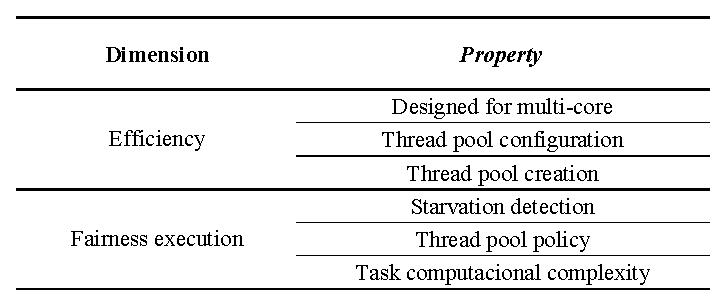
\includegraphics[scale=0.9]{./figs/issues.eps}
	%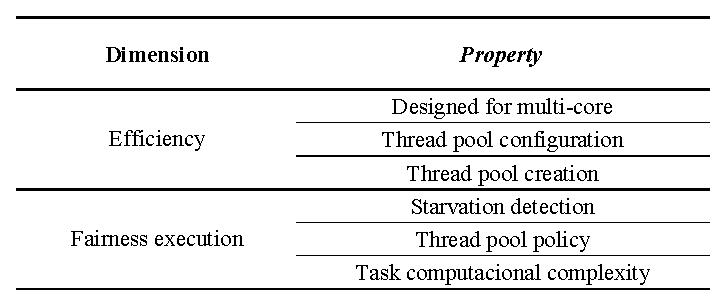
\includegraphics[width=\linewidth]{./figs/issues.eps}
\label{tab:problems}%
\end{table}%
%==============================================================================
\subsubsection{{Directions on Efficiency}}
\label{subsubsec:directions_efficiency}
%==============================================================================
Software engineers seek to develop algorithms that can take full advantage of multi-core design so that achieve a high level of parallelism and an overall high performance. The way the algorithms are written impact in the success of multi-core technology strongly~\cite{sethi2015}. Design multi-core is a property, which should be present in runtime systems bearing in mind that the technological advances already offers resources to extends the parallel program. For hardware, we can cite the modern technologies Graphics processing units (GPUs), which demand tens of thousands of concurrent threads to fully utilize the massive amount of processing resources~\cite{yoon2016}. GPUs hold great massively parallel computing capabilities, with potential for the acceleration of computationally intensive algorithms~\cite{tang2017}. 

Some works are shown promising proposals of thread pool configuration models, like the article of Nazeer et al.~\cite{nazeer2016}, which achieves good results in simulations, with the named Hybrid scheme to dynamically, which optimize a thread pool, based on predicting incoming request frequencies. Gleyzer et al.~\cite{gleyzer2017} propose a method allows dynamic thread pool sizing suitable for use in multi-threaded processing environment such as a distributed data grid. The method utilizes measurements of thread pool throughput and measurements of worker thread utilization in combination with analysis of prior thread pool resizing actions to determine whether to add or remove worker threads from a thread pool in a current resizing action. The method claims a rapid and responsive adjustment of thread pool size in response to changes in workload and processor availability. These works motivate us to deepen our research, so that the thread pool configuration of the runtime systems of the integration platforms occurs elastically, following the demand of processing the tasks and thus, using the computational resources more efficiently.

The research of Lee et al.~\cite{lee2011} shows better response time and CPU usage, by means prediction of the number of threads and thread pool management. Trendy exponential moving average (TEMA) scheme, proposed by Lee et al., adjusts the idle time out period and thread pool size to adapt the system to the changing environment. The article of Oh and Kim~\cite{oh2013} presents a history-based dynamic method (HisDyn), which minimizes throughput degradation, due to creation of threads, by means of estimation and maintenance of the number of threads needed for requests. HisDyn predicts the range of needed threads, through of the mean task arrival times and mean task processing times.

Bahadur et al.~\cite{bahadur2014} propose a thread pool system able of dynamic optimization thread pool size, according request frequencies, named Frequency Based Optimization Strategy (FBOS). After, Ashraf et al.~\cite{ashraf2016} present an extension of work of FBOS, namely Non-blocking Frequency Based Optimization Strategy with Automated Timers (NBFBOS with Automated Timers), which dynamically optimises thread pool, using of non-blocking synchronization primitives offering advantages of substantial scalability and liveliness. For all this, we believe that it is possible to find out to get optimised strategies to create threads at runtime to runtime systems of integration platforms.

%==============================================================================
\subsubsection{{Directions on Fairness execution}}
\label{subsubsec:directions_fairness}
%==============================================================================
Shah et al.~\cite{shah2017} argue that when starvation occurs it decreases response time and increases wait time to execution of requests and propose to explore the implementation of multiple thread pools based on a distribution of service times to avoid starvation and achieve concurrency of processing. Their analysis showed that proposed scheme is increases the response time and reduces the wait time. This research endorses the need and possibility of the runtime systems detecting starvation detection, therefore, the detection starvation is a potential field of study.

Tsai et al.~\cite{tsai2013} propose to optimize task scheduling and resource allocation using an improved differential evolution algorithm (IDEA), based on the proposed cost and time models on cloud computing environment. Elmougy et al.~\cite{elmougy2017} propose a novel hybrid task scheduling algorithm named (SRDQ) combining Shortest-Job-First (SJF) and Round Robin (RR) schedulers considering a dynamic variable task quantum. Singh et al.~\cite{singh2017} present a review of using meta-heuristics techniques for scheduling tasks in cloud computing, based on swarm intelligence and bio-inspired techniques and claim that it is possible to decide suitable approach for better schemes for scheduling according to the application. These works encourages us to pursue smarter policies to schedule tasks for the thread pools in the runtime systems of integration platforms.

Cordes et al.~\cite{cordes2011} claim that it is essential to balance the execution time of all tasks in a work flow of processing running in parallel in order to achieve the best possible utilization of computing resources. The proposed method by authors employs a cost model that allows incorporating differing execution times for loop iterations of the program due to the underlying heterogeneous platform. The consideration of execution time heterogeneity enables the in parallel approach to using each processing unit according to its performance characteristics in a system as well as the utilization of as many processing units as possible simultaneously.

The research of Sudarsanam et al.~\cite{sudarsanam2004} address the compatibility between resource and task by estimating the amount of resources that are needed for a reconfigurable architecture to suit task granularity. These studies point out that considering the computational complexity to be executed can lead to a better allocation of computational resources.
